\chapter{Methodology}

\section{Hasing module}

\subsection{Test Setup}
In order to evaluate the performance increase obtained when using a dedicated
hashing accelerator, a test system was constructed using Xilinx' Vivado
development studio.

\begin{figure}[ht]
	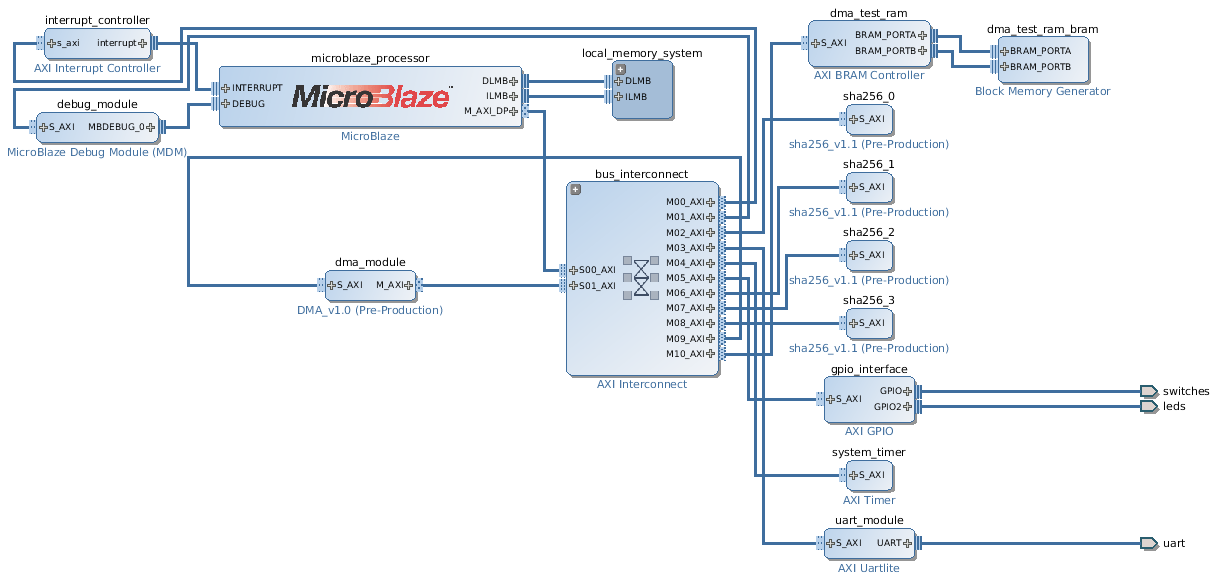
\includegraphics[width=0.95\textwidth]{Figures/testsystem-vivado.png}
	\caption{Overview of the test system}
	\label{fig:testsystem-vivado}
\end{figure}

The test system is controlled by a MicroBlaze microprocessor, configured to
include the optional barrel shifter, integer divider and pattern comparator.
In order to run the XilKernel real-time operating system, the system also
includes a simple timer module for use by the kernel.

A UartLite module was included to provide I/O in order to communicate with
the system from a desktop computer, as well as a GPIO module for additional
debugging use.

The system runs on a 50~MHz clock which is synthesized by a clock generator
module from a 100~MHz input clock.

In order to run performance tests on the system, the DMA described in
section \ref{undefined}\todo{Insert correct reference here} and four
SHA256 hashing modules are included.\todo{Maybe reduce to one now}
A fixed-interval timer, that generates an interrupt every second, is
included in order to calculate the performance per second.

\subsection{Test Software}
In order to test the hashing modules and how the performance scales when including
multiple hashing modules, a benchmark application was written. The benchmark
runs a specified number of threads that tries to hash a single block of data
over and over again.

A simple scheduler is used to provide each thread with an available hashing module.
If no module is available, the thread blocks on a semaphore until a module is available.

Once a second, the number of completed hashes for each module is added up and
reported over the UART.

The test software is also designed so that it can be run with a software implementation
of the hashing algorithm instead of the hashing modules. This makes it possible
to compare the performance when using an accelerator as compared to not using
an accelerator.

\subsection{Measurements and Benchmarks}
The most important performance measure for a Bitcoin mining system is the number
of hashes per second it can sustain. Therefore, once a second the number of hashes
computed since the previous second is calculated and sent over the UART.

Another important measurement is how the inclusion of a DMA affects the performance
of the system.

\subsection{Theoretical Maximum Performance} % This section can be moved elsewhere

The hashing modules can finish one round of hashing in 65 clock cycles. If
every hash can be obtained from only one block of data, it is possible to
obtain a hash every 65 clock cycles under ideal conditions. This translates
into a maximum theoretical performance of 768230~H/s at a clock frequency of
50~MHz.

However, the modules do not exist in a vacuum, and data needs to be transferred
between the modules and a controller, such as a microprocessor. The hashing tiles
are connected to the rest of the system using an AXI4 lite interface. Transfers
on the AXI bus takes at least three cycles for writes and two cycles for reads,
if it is assumed that no burst transfers are used\footnote{Indeed, the AXI4 lite
interface only allows burst lengths of one word, in essence no burst transfer is
supported.}

In order for the hashing module to word, it needs 16 32-bit words of input data,
and control signals must be set up. This causes at least 17 words of data to
need to be written to the module, taking at least 51 clock cycles. Then, after
hashing of a block is complete, if there are no more blocks, the result must
be read back. The result consists of 8 words of data, which takes at least 16
clock cycles to transfer.

In total, a minimum of 67 clock cycles of overhead is needed per hash when assuming
a one-block input size and an ideal AXI4 bus. Not considering the additional overhead
from processing in the microprocessor, such as when handlig the interrupt when the
hashing finishes, hashing may take a minimum of $67 + 65 = 132$ clock cycles to
complete, bringing the maximum theoretical performance down to at most 378787~H/s.

However, in a real system, there are many additional sources of overhead reducing
the performance additionally.\todo{Maybe move this somewhere else}

\subsection{Testing performance of DMA Module}

In the system set up for this project, a load takes at least 2 cycles, and a store takes at least 3 cycles.
Branching and incrementation takes at least 1 cycle each.
For M data, the total transfer for the CPU takes at least 
\\ (3 + 2 + 1 + 1) * M = 7M cycles, for the loop only.
\\ If a DMA module is present, it can relieve the CPU for this work, letting the CPU focus on another work, saving it 7M cycles for each transfer, with exception of overhead, such as activating the DMA Module and handling interrupts when done.
In addition, a well designed DMA Module may have less overhead, enabling better \todo{With more than one channel active, a transfer does not necessarily become faster by itself} throughtput.

A program with M data to be transfered will be used, and the number of clock cycles spent on other work than data transfer for the CPU will be measured.
A comparison with running with and wihtout DMA Module will be done, to see the CPU can spend at least 7M more cycles of work on other tasks.
This does not include data loads/stores the CPU needs for itself.

In addition, the hashing module will be tested with using the DMA Module for data transfer, to see if adding DMA Module improves the overall performance for the hashing module.